\documentclass[11pt,nswissgerman]{article}
\usepackage{helvet}
\renewcommand{\familydefault}{\sfdefault}
\usepackage[latin2]{inputenc}
\usepackage[a4paper]{geometry}
\geometry{verbose,tmargin=3cm,bmargin=3cm,lmargin=3.5cm,rmargin=3.5cm,headheight=3cm,headsep=1cm,footskip=2cm}
\usepackage{fancyhdr}
\pagestyle{fancy}
\usepackage{wrapfig}
\usepackage{graphicx}
\usepackage[position=bottom]{subfig}
\usepackage{titletoc}
\usepackage{float}
\makeatletter
\@ifundefined{date}{}{\date{}}
\makeatother
\usepackage{babel}
\usepackage[
            colorlinks=true,
            urlcolor=green,
            linkcolor=black
]{hyperref}
\setcounter{secnumdepth}{1} % levels under \section are not numbered
\setcounter{tocdepth}{2}    % levels under \subsection are not listed in the TOC
\begin{document}
\author{Stefan Bopp}
\title{\Huge Ostern in Walenstadt 2017\vspace{2cm}

\includegraphics[width=0.4\textwidth]{../Bilder/Logo/Logo.png}
}
\maketitle
\vfill
\tableofcontents

\newpage

\lhead{Walenstadt 2017}

\rhead{jackthebus.com}

\cfoot{\thepage}
\subsection{14.04.2017 Anreise}
\begin{wrapfigure}{R}{0.45\textwidth} 
  \begin{centering}
    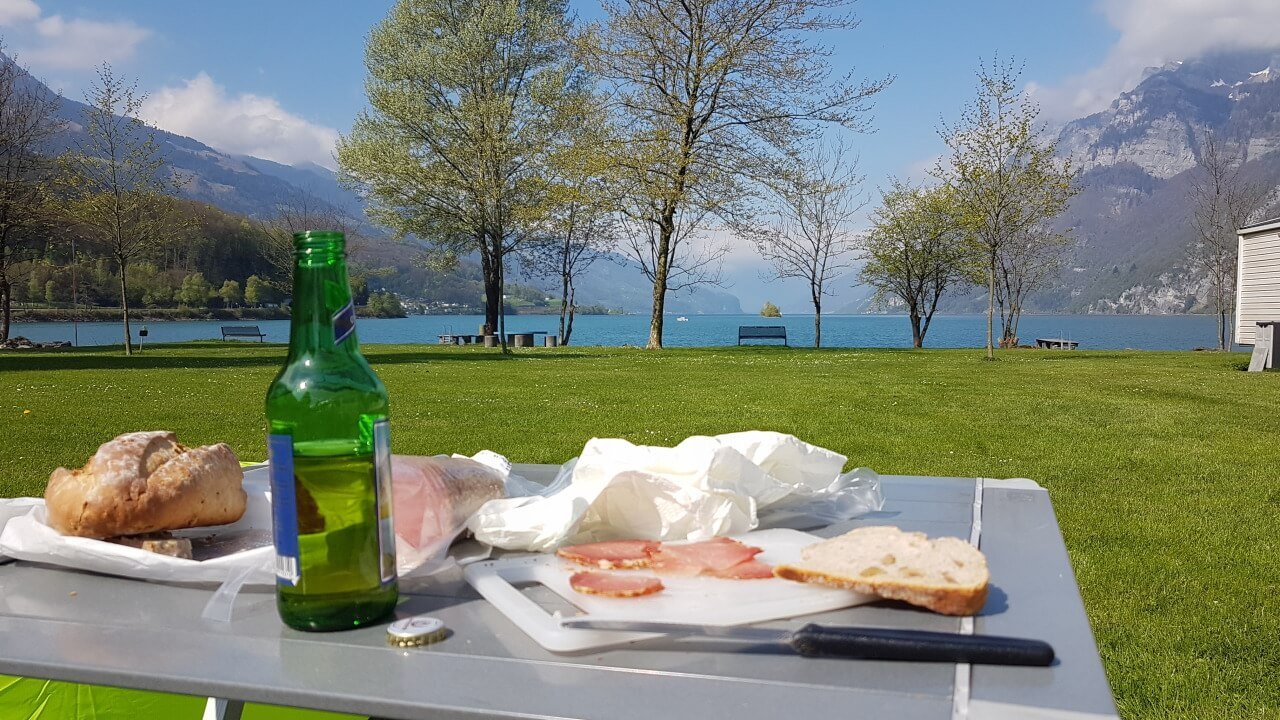
\includegraphics[width=0.4\textwidth, height=5cm, keepaspectratio]{../Bilder/Walensee/7.jpg}
    \caption{Picknick am Walensee}
  \end{centering}
\end{wrapfigure} 

\begin{figure}[b]
\centering
      %\subfloat[CAPTION]{BILDERCODE}\qquad
   \subfloat{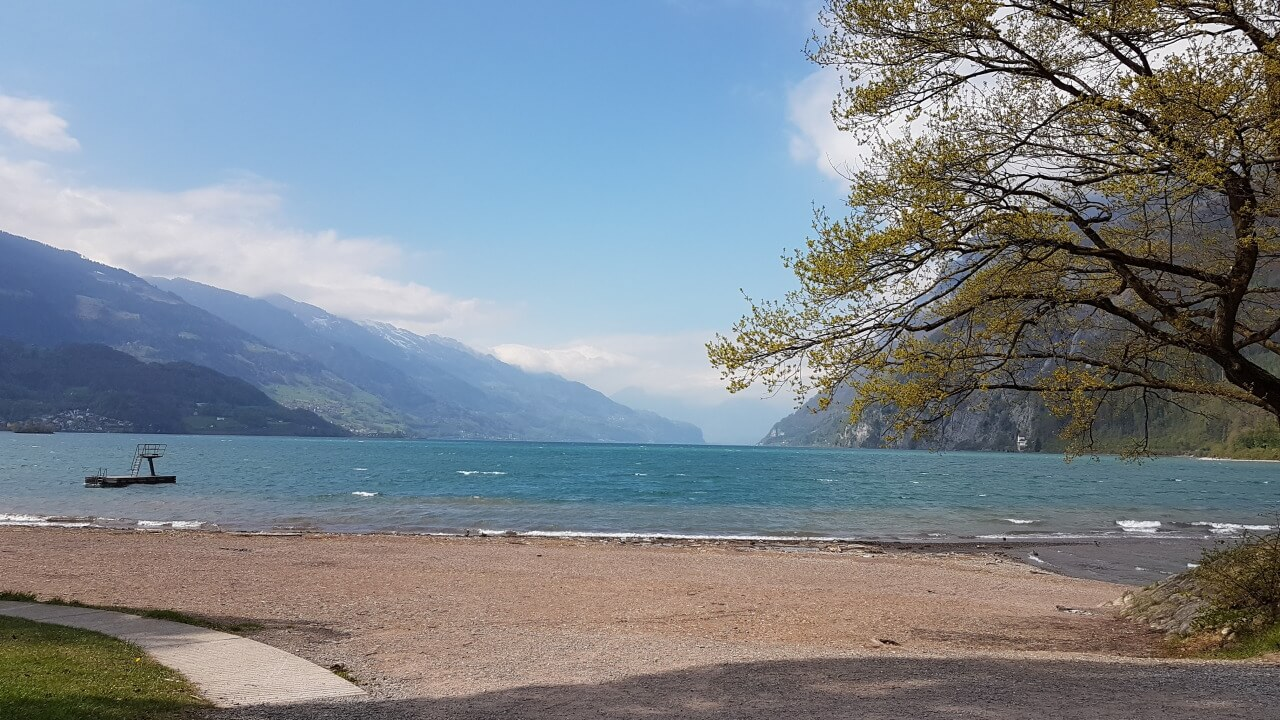
\includegraphics [width=0.3\textwidth]{../Bilder/Walensee/9.jpg}}\quad
   \subfloat{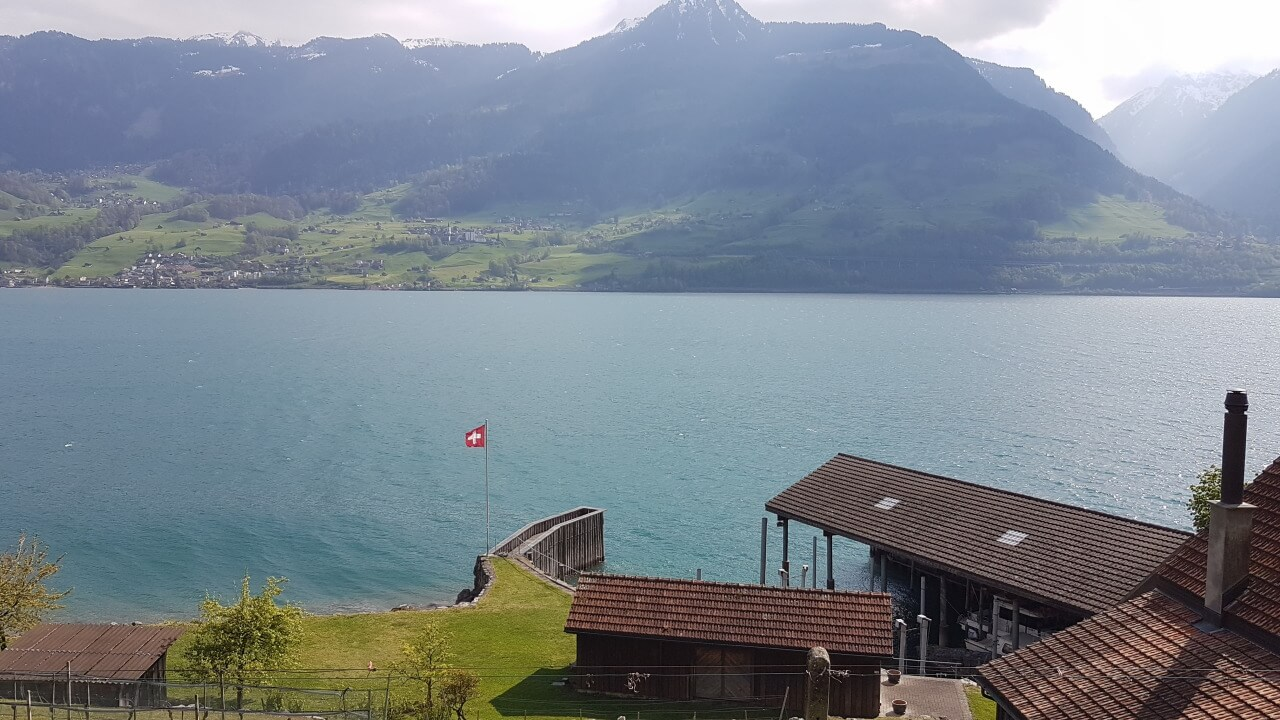
\includegraphics [width=0.3\textwidth]{../Bilder/Walensee/22.jpg}}\quad
   \subfloat{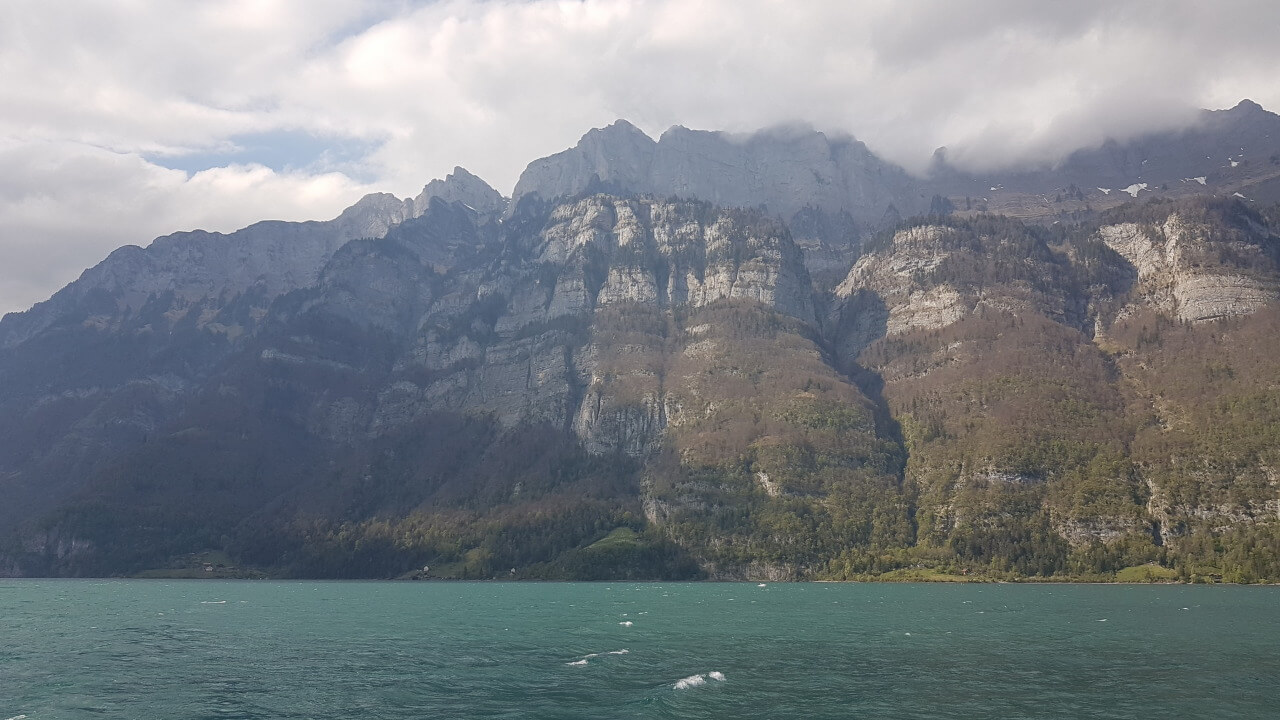
\includegraphics [width=0.3\textwidth]{../Bilder/Walensee/24.jpg}}\quad
   \caption[Wanderung am Walensee]{Wanderung am Walensee}
\end{figure}

Die Wetterprognosen und die Staul�nge vor dem Gotthard motivierten f�r ein fr�hes Aufbrechen.
Das allj�hrliche vor dem Gotthardtunnel stehen hatte sich schon auf rekordverd�chtige 14 Kilometer hoch gestanden was �bersetzt hiess, dass das Wetter im Norden eher bescheiden sein wird.
Doch der Karfreitag versprach aus der Reihe zu tanzen.
Wolkenloser Himmel begr�sste uns und so machten wir uns kurz nach sieben bepackt mit Velos und dem n�tigsten auf den Weg nach Nussbaumen, dem Heim unseres Busses. 
Nach dem Umladen der sieben Sachen und einem kurzen Halt um die Autobahn-Vignette zu kaufen sowie Treibstoff zu tanken ging es Richtung Z�rich.
Das Wetter war bei der Abfahrt in Luzern um einiges besser als im Flachland.
Gl�cklicherweise verkehrte sich der Effekt wieder als wir wiederum Richtung Alpen fuhren.
Kurz nach dem Z�richsee zeigte sich das Wetter wieder von der besten Seite.
Die vielen Tafeln, welche vorschlugen den San Bernadino als Alternative zu benutzen zeigten noch keine Wirkung
und so konnten wir ohne Stau bis fast an den Walensee fahren.
Kurz nach Weesen hatten sich mehrere Fahrzeuge zur Kaltverformung zusammengefunden, wir hatten jedoch Gl�ck und standen da maximal 10 Minuten.
Kurz darauf befanden wir uns auf der Ausfahrt Walenstadt.
Die Saison startete just heute f�r den Campingplatz See Camping.
Zus�tzlich machten die miesen Wetterprognosen dem erwarteten Andrang einen Strich durch die Rechnung.
Die Auswahl der Stellpl�tze machte die Qual der Wahl nicht einfacher.
Direkt am See genossen wir so einen Imbiss bei sch�nstem Sonnenschein.

Noch heute, um das gute Wetter zu nutzen, sollte es auf grosse Wanderung gehen.
Dem Ufer des Walensee entlang nach Quinten oder Aue.
Der Walensee hat jedoch ziemlich steile Ufer, somit waren wir gezwungen einige H�henmeter in Kauf zu nehmen um dem Ufer zu folgen.
Nach einem netten Schwatz mit einer Eingeborenen ging die Wanderung 500m �ber dem Walensee weiter.
Die einzige M�glichkeit sich den R�ckweg per pedes zu ersparen bot das Kursschiff, welches
heute auch wieder den Betrieb aufnahm.
Dieses galt es unter keinen Umst�nden zu verpassen.
Unterwegs bemerkten wir, dass wir dank gutem Vorankommen Chancen haben das fr�here Schiff zu erreichen und so vor dem Essen noch Duschen zu k�nnen.
Nach der kurzen Fahrt �ber den Walensee kamen wir an der sch�nen Uferpromenade in  Walenstadt an, welche sich wegen dem aufkommenden Wind schon massiv entv�lkert hat.
Nach einem Ap�ro marschierten wir zur�ck zum Camping um nach einer Dusche die Fahrr�der zu
satteln um uns einen feinen Fisch im Restaurant Seehof zu g�nnen.
Nach der R�ckkehr zum Bus schalteten wir die Standheizung in den Modus "`Sauna"'.
Dementsprechend unruhig war die erste Nacht des Jahres 2017 im Bus.


\subsection{15.04.2017 Fashion Outlet und B�ndner Herrschaft}

\begin{wrapfigure}{L}{0.45\textwidth} 
  \begin{centering}
    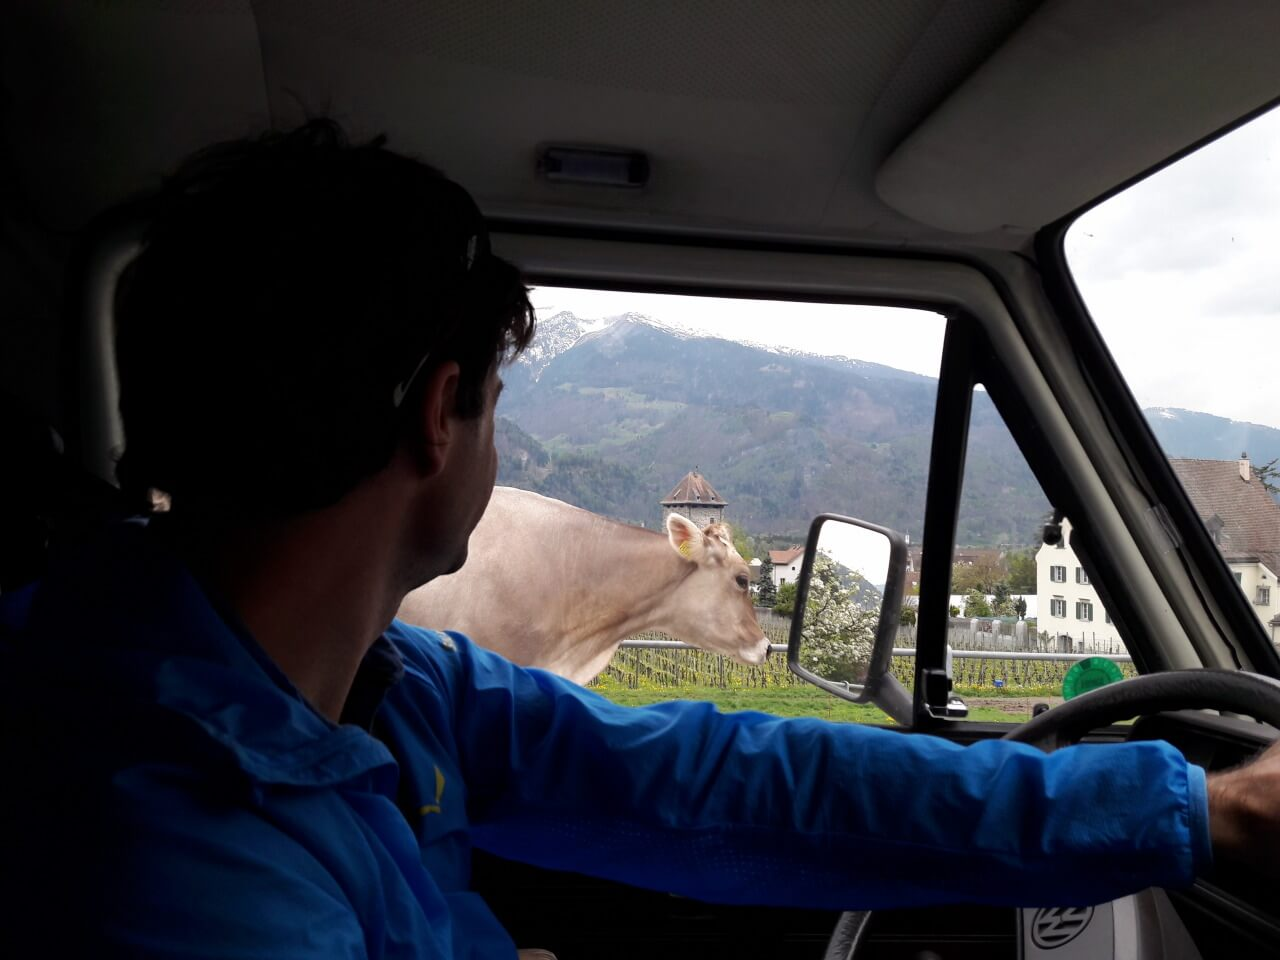
\includegraphics[width=0.4\textwidth, height=5cm, keepaspectratio]{../Bilder/Walensee/28.jpg}
    \caption{Kuh macht Ausflug}
  \end{centering}
\end{wrapfigure}

Nach einer eher unruhigen Nacht blinzelte schon fr�h die Sonne durch die Vorh�nge was eigentlich so gar nicht vorgesehen war.
Der Wetterbericht war eher negativ und so beschlossen wir das  Fashion Outlet in Landquart unsicher zu machen.
Der Bus wurde nach dem Fr�hst�ck fahrbereit gemacht und kurz darauf befanden wir uns auf der Fahrt Richtung Chur.
Der Weg wurde genutzt um unsere weiteren kulinarischen Pl�ne in die Tat umzusetzen.
Wie meistens �blich wurden wir nach Bekanntgabe des Reiseziels mit sehr guten Tipps aus D�ttwil �bersch�ttet, welche Restaurants in der Gegend einen Besuch wert sind.
Aus diesem Grund sollte am Abend Murg angesteuert werden. 
F�r die Eskalation im Fashion Outlet sorgte dann eher der untypische Teil eines Paares.
Ich tauchte schlussendlich schleppend wieder beim Bus auf und pr�sentierte Stolz meinen Fang.
Pfannenset, Zubeh�r und Bratpfannen haben es mir angetan.
B�se Zungen behaupten das Liege in der Familie�
Der Himmel zog sich immer mehr zu und trotzdem wollten wir es nicht missen einen Blick auf die wundersch�nen D�rfer in der B�ndner Herrschaft zu werfen.
So durchquerten wir Malans, Jenins, Maienfeld und Fl�sch und tr�umten von w�rmeren Wetter und langen Abenden in den Torkel und Reben der Gegend. 
Dank dem sehr gut ausgebauten �V-Netz beschlossen wir den Bus f�r das Nachtessen stehen zu lassen und mit dem Bus nach Murg zu fahren.
Da wir noch eher fr�h dran waren konnten wir noch kurz das zum Restaurant geh�rendem Lodge Hotel besuchen.
Nach einem Ap�ro hatten gewisse Teile der Crew von Jack schon wunderbar eines am Helm.
Das echt sehenswerte Restaurant versorgte uns mit wunderbaren K�stlichkeiten und der gute Wein tat den Rest  um den Abend zu einem Erfolg werden zu lassen.
Die Heimfahrt verging dann dank promillebedingter Bet�ubung wie im Flug.
Etwas muss jedoch noch erw�hnt werden: Ich wusste gar nicht, dass am Bahnhof in Murg auch Dampfschiffe fahren.
Das Nebelhorn war auf jeden Fall gut zu h�ren.

\begin{figure}[H]
    \centering
    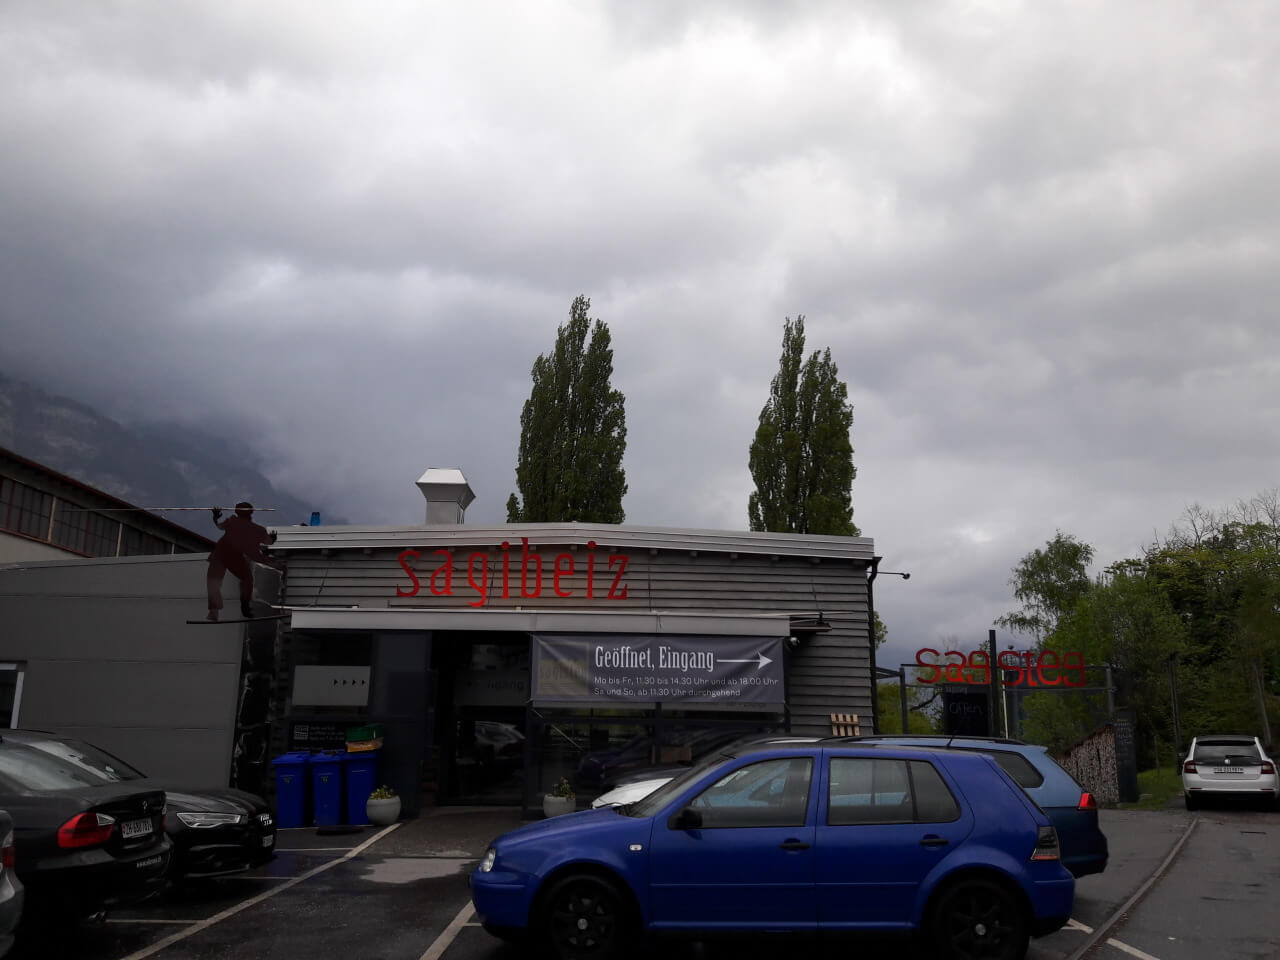
\includegraphics[width=\textwidth]{../Bilder/Walensee/31.jpg}
    \caption{Sagibeiz in Murg}
    \label{img:Sagibeiz}
\end{figure}

\subsection{16.04.2017 Bad Ragaz} 
Das gleichm�ssige Ger�usch versprach nichts Gutes.
Es regnete und so sollte es denn ganzen Tag auch weitergehen.
Schon das Fr�hst�ck im Bus war eine Herausforderung und so kam bald einmal die Frage auf ob wir heute abfahren sollten oder noch eine Nacht �ausharren� sollten.
Die sprichw�rtliche Bequemlichkeit entschied dann f�r uns und wir machten es uns im Bus gem�tlich und planten den Besuch in der Tamina Therme in Bad-Ragaz.
Wenn schon Nass dann wenigstens 36.5�.
Tats�chlich hatte das Wetter kein Erbarmen und es regnete ununterbrochen weiter.
Nach einem Imbiss in der B�ckerei kamen wir durchn�sst bei der Therme an.
Die n�chsten 2 Stunden hiess es t�chtig aufw�rmen und das sprudelnde Wasser geniessen, bevor uns ein weiteres Mal das eiskalte Wetter begr�sste.
Der Spaziergang vom Bahnhof Walenstadt zum Campingplatz war dieses Mal besonders lang. 
Alles durchn�sste wurde behelfsm�ssig im Bus verteilt, so dass die Standheizung ihren Dienst tun konnte.
Das machte sie auch prompt und schon bald hatten wir eine Art k�nstliche Tropfsteinh�hle im Bus.
Erinnerungen an den Ausflug nach �geri wurden wach.
Das warme Wasser von Bad-Ragaz sowie das schlechte Wetter machten die Entscheidung leicht nicht mehr f�r das Abendessen auszugehen.
Somit war heute Ravioli Abend, was nicht gerade f�r Begeisterungsst�rme seitens Chantal sorgte.
Die mitgebrachten Serien auf dem Laptop hatten ein leichtes Spiel uns in den Schlaf zu begleiten.

\subsection{17.04.2017 Zusammenpacken und R�ckfahrt}
Gl�cklicherweise hatten wir eine Regenstopp der dazu genutzt werden konnte unsere Siebensachen einzupacken und uns auf den Weg Richtung Rastst�tte Glarnerland zu machen.
Die Churfirsten welche uns am Freitag noch fr�hlingshaft begr�ssten, waren bei der Abfahrt wieder bis weit nach unten mit einer feinen Schneeschicht �berzogen.

Die Region Walensee, wir werden sie garantiert ein weitere Mal besuchen...

\begin{figure}[H]
    \centering
    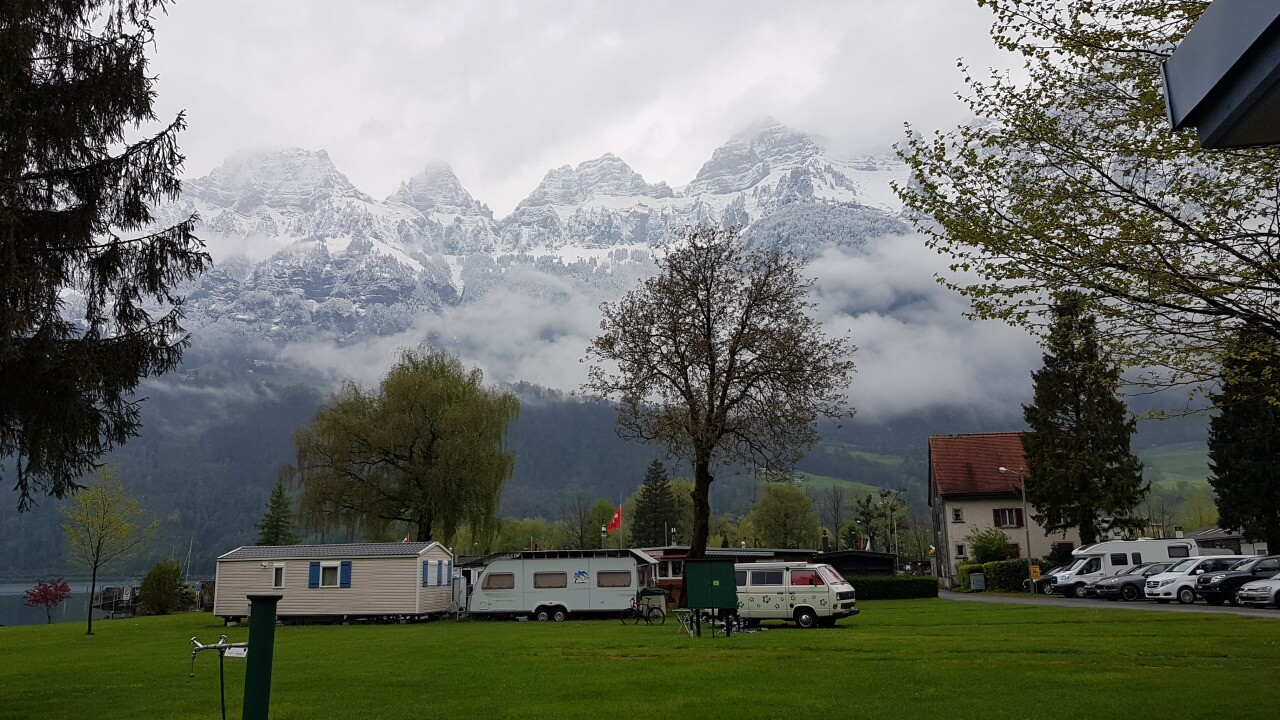
\includegraphics[width=\textwidth]{../Bilder/Walensee/35.jpg}
    \caption{Wieder verschneite Churfirsten}
    \label{img:Churfirsten}
\end{figure}

\newpage

\begin{figure}[H]
    \centering
    
\includegraphics[width=\textwidth,height=14cm, keepaspectratio]{../Bilder/Logo/Logo_trans.png}
    \label{img:Logo}
\end{figure}
\vfill
    \begin{center}
        {\huge  Weitere Informationen zum Bus und unseren Reisen sind auf der Homepage {\url{www.jackthebus.com}} zu finden}
\end{center}

\end{document}
